\immediate\write18{tex spath3_code.dtx}
\documentclass{ltxdoc}
\usepackage[T1]{fontenc}
\usepackage{trace}
\usepackage{lmodern}
\usepackage{morefloats}
\usepackage{tikz}
\usetikzlibrary{knots,spath3,hobby}
\usepackage[numbered]{hypdoc}
\definecolor{lstbgcolor}{rgb}{0.9,0.9,0.9} 
 
\usepackage{listings}
\lstloadlanguages{[LaTeX]TeX}
\lstset{
  breakatwhitespace=true,
  breaklines=true,
  language=[LaTeX]TeX,
  basicstyle=\small\ttfamily,
  keepspaces=true,
  columns=fullflexible
}
 
\usepackage{fancyvrb}

\newenvironment{example}
  {\VerbatimEnvironment
   \begin{VerbatimOut}{example.out}}
  {\end{VerbatimOut}
   \begin{center}
   \setlength{\parindent}{0pt}
   \fbox{\begin{minipage}{.9\linewidth}
     \lstinputlisting[]{example.out}
   \end{minipage}}

   \fbox{\begin{minipage}{.9\linewidth}
     \centering
     \input{example.out}
   \end{minipage}}
\end{center}
}

\providecommand*{\url}{\texttt}
\GetFileInfo{spath3.sty}

\title{The \textsf{knots} Package: Documentation}
\author{Andrew Stacey \\ \url{loopspace@mathforge.org}}
\date{\fileversion~from \filedate}

\begin{document}

\maketitle

\section{Pre-Introduction}

This library is built on top of a package for manipulating PGF's \emph{soft paths} called \texttt{spath3}.
  Version 2.0 of \texttt{spath3} involved considerable reorganisation of the code.
  I tried to ensure that this didn't affect this library but it is extremely likely that I wasn't fully successful.
  If something that used to work no longer does, please do let me know either by opening an issue on github (\url{https://github.com/loopspace/spath3}) or at the above email.

  That version of \texttt{spath3} also introduced an alternative way of drawing knots which involves breaking the paths at their crossing points and introducing actual gaps.
  This makes it easier to do things like have the knots on non-uniform backgrounds, and to style different parts of the knot differently such as illustrating a \(3\)--colouring.
  To see how that works, look at the documentation of the \texttt{spath3} TikZ library.
  Here's an example of how to draw a knot with that library.

  \begin{example}
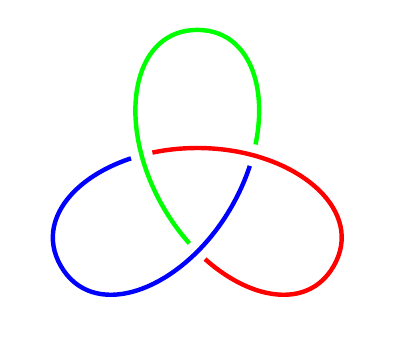
\begin{tikzpicture}[
    use Hobby shortcut,
    every trefoil component/.style={ultra thick, draw},
    trefoil component 1/.style={red},
    trefoil component 2/.style={blue},
    trefoil component 3/.style={green},
]
\path[spath/save=trefoil] ([closed]90:2) foreach \k in {1,...,3} { .. (-30+\k*240:.5) .. (90+\k*240:2) } (90:2);
\tikzset{spath/knot={trefoil}{8pt}{1,3,5}}
\end{tikzpicture}
\end{example}


\section{Introduction}
  
The \Verb+knots+ package is a TikZ library for drawing knot (and similar) diagrams.
It provides a few useful styles and node shapes but its main contribution is the \Verb+knot+ environment.
The \Verb+knot+ environment allows you to draw some strands of a knot (or braid or tangle or whatever -- we shall use the imprecise term ``knot'' to refer to any similar diagram) and then to modify the crossings via a simple interface.

The main part of this package was developed in response to a question on the \href{http://tex.stackexchange.com}{TeX-SX} site by Jamie Vicary.
The original question was \href{http://tex.stackexchange.com/q/32125/86}{Braid diagrams in TikZ}.
Jamie's comment (quoted below) was the inspiration for the mechanism of the \Verb+knot+ environment.

\begin{quotation}
[It] would be really cool if it was possible to draw the curves, let TikZ calculate all the intersection points automatically, and then tell it to redraw the intersections according to an under/over specification... do you think this is in the realm of plausibility?
\end{quotation}

\section{Examples}

Let us begin with an example.
To use the library, simply load the \Verb+tikz+ package and add \Verb+knots+ to the list of TikZ libraries that you load.
For example, the following in your preamble would work:

\begin{verbatim}
\usepackage{tikz}
\usetikzlibrary{knots}
\end{verbatim}

Let's draw a simple tangle (actually a braid).

\begin{example}
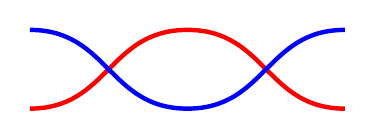
\begin{tikzpicture}
\draw[red,ultra thick] (0,0) .. controls +(1,0) and +(-1,0) .. (2,1) .. controls +(1,0) and +(-1,0) .. (4,0);
\draw[blue,ultra thick] (0,1) .. controls +(1,0) and +(-1,0) .. (2,0) .. controls +(1,0) and +(-1,0) .. (4,1);
\end{tikzpicture}
\end{example}

Now a common way to draw crossings for knots is to draw a gap in the under strand through which the over strand passes.
One way to achieve this in TikZ is to draw the over strand twice, the first time with a thicker line width and the colour of the background.
We'll draw it twice, once with background a different colour to illustrate this.

\begin{example}
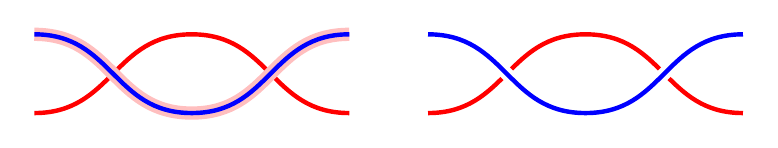
\begin{tikzpicture}
\draw[red,ultra thick] (0,0) .. controls +(1,0) and +(-1,0) .. (2,1) .. controls +(1,0) and +(-1,0) .. (4,0);
\draw[pink,double=blue,ultra thick,double distance=1.6pt] (0,1) .. controls +(1,0) and +(-1,0) .. (2,0) .. controls +(1,0) and +(-1,0) .. (4,1);
\draw[xshift=5cm,red,ultra thick] (0,0) .. controls +(1,0) and +(-1,0) .. (2,1) .. controls +(1,0) and +(-1,0) .. (4,0);
\draw[xshift=5cm,white,double=blue,ultra thick,double distance=1.6pt] (0,1) .. controls +(1,0) and +(-1,0) .. (2,0) .. controls +(1,0) and +(-1,0) .. (4,1);
\end{tikzpicture}
\end{example}

Now the problem with this method is that there is no way to draw the red and blue paths so that the blue is the over strand at the first crossing and the red at the second.
Either the blue path is always on top (as shown) or the red.
One way to resolve this is to split the paths and draw one of them in segments:

\begin{example}
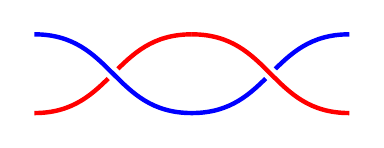
\begin{tikzpicture}
\draw[red,ultra thick] (0,0) .. controls +(1,0) and +(-1,0) .. (2,1);
\draw[white,double=blue,ultra thick,double distance=1.6pt] (0,1) .. controls +(1,0) and +(-1,0) .. (2,0) .. controls +(1,0) and +(-1,0) .. (4,1);
\draw[white,double=red,double distance=1.6pt,ultra thick] (2,1) .. controls +(1,0) and +(-1,0) .. (4,0);
\end{tikzpicture}
\end{example}

Another method (employed by the \Verb+braids+ package) is to break the under path either side of the crossing and not draw it there.
This means that the order of drawing doesn't matter.

Both of these methods have their drawbacks (particularly for general knots as opposed to the more structured braids) in that they require a detailed knowledge of the pieces of the paths and the positions of the crossings.
As pointed out by Jamie Vicary in the above-{}quoted comment, TikZ should be able to compute these itself.

That's what this package does.

Let's do the above example using this package.
The main changes to the drawing are that we use the command \Verb+\strand+ rather than \Verb+\draw+ and we enclose it in the \Verb+knot+ environment.
When initially drawing the strands it is useful to provide the option \Verb+draft mode=strands+.
That's because the detailed computation can take a little time and so it is best only to do it when necessary.
So on first run through we get the following.

\begin{example}
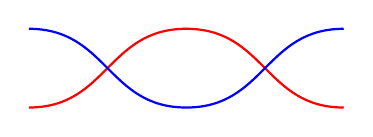
\begin{tikzpicture}
\begin{knot}[
  draft mode=strands
]
\strand[red,thick] (0,0) .. controls +(1,0) and +(-1,0) .. (2,1) .. controls +(1,0) and +(-1,0) .. (4,0);
\strand[blue,thick] (0,1) .. controls +(1,0) and +(-1,0) .. (2,0) .. controls +(1,0) and +(-1,0) .. (4,1);
\end{knot}
\end{tikzpicture}
\end{example}

Once we're happy with the positioning of the strands, we change the option \Verb+draft mode=strands+ to \Verb+draft mode=crossings+.

\begin{example}
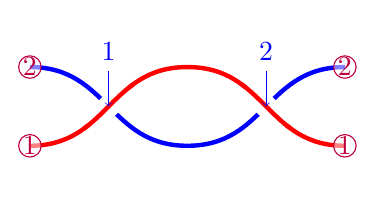
\begin{tikzpicture}
\path (2,1.5) (2,-.5);
\begin{knot}[
  draft mode=crossings,
  clip width=5,
]
\strand[red,ultra thick] (0,0) .. controls +(1,0) and +(-1,0) .. (2,1) .. controls +(1,0) and +(-1,0) .. (4,0);
\strand[blue,ultra thick] (0,1) .. controls +(1,0) and +(-1,0) .. (2,0) .. controls +(1,0) and +(-1,0) .. (4,1);
\end{knot}
\end{tikzpicture}
\end{example}

The \Verb+\path (2,1.5) (2,-.5);+ is to extend the bounding box of the picture a little upwards.
The extra pieces are not used when computing the bounding box of the picture so that it doesn't change position on the page.

The extra information is that the strands and the crossings have been numbered.
The crossings have also been rendered (the \Verb+clip width+ option enlarges the crossing gap to make it more obvious).
Unfortunately, for both crossings the red path is on top.
We need to flip one of these crossings (the first).
To do this, we either use the command \Verb+flipcrossings+ or the \Verb+flip crossing+ key. 

\begin{example}
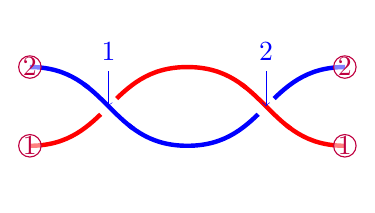
\begin{tikzpicture}
\path (2,1.5) (2,-.5);
\begin{knot}[
  draft mode=crossings,
  clip width=5,
  flip crossing=1,
]
\strand[red,ultra thick] (0,0) .. controls +(1,0) and +(-1,0) .. (2,1) .. controls +(1,0) and +(-1,0) .. (4,0);
\strand[blue,ultra thick] (0,1) .. controls +(1,0) and +(-1,0) .. (2,0) .. controls +(1,0) and +(-1,0) .. (4,1);
\end{knot}
\end{tikzpicture}
\end{example}

Once we're happy with it, we remove the \Verb+draft mode+ option to render it in its final form.

\begin{example}
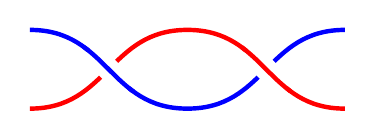
\begin{tikzpicture}
\begin{knot}[
  clip width=5,
  flip crossing=1,
]
\strand[red,ultra thick] (0,0) .. controls +(1,0) and +(-1,0) .. (2,1) .. controls +(1,0) and +(-1,0) .. (4,0);
\strand[blue,ultra thick] (0,1) .. controls +(1,0) and +(-1,0) .. (2,0) .. controls +(1,0) and +(-1,0) .. (4,1);
\end{knot}
\end{tikzpicture}
\end{example}

Here's a more complicated example.

\begin{example}
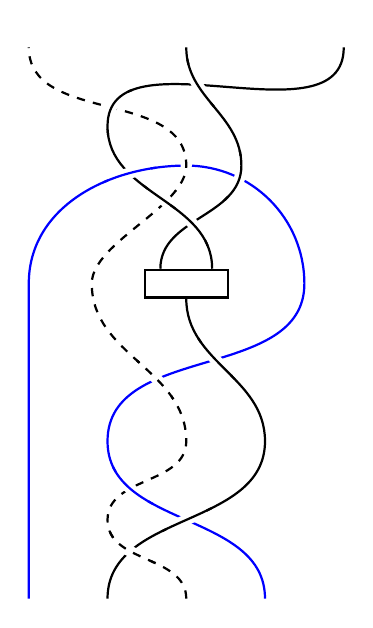
\begin{tikzpicture}
\node (A) at (0,4) [draw,minimum width=30pt,minimum height=10pt,thick] {};
\begin{knot}[
  clip width=5,
  clip radius=8pt,
]
\strand [thick,only when rendering/.style={dashed}] (0,0)
to [out=up, in=down] (-1,1)
to [out=up, in=down] (0,2)
to [out=up, in=down] (-1.2,4)
to [out=up, in=down, looseness=0.7] (0,5.5)
to [out=up, in=down] (-2,7);
\strand [thick] (-1,0)
to [out=up, in=down] (1,2)
to [out=up, in=down] (A.south);
\strand [thick,blue] (1,0)
to [out=up, in=down] (-1,2)
to [out=up, in=down] (1.5,4)
to [out=up, in=right] (0,5.5)to [out=left, in=up] (-2,4)
to [out=down, in=up] (-2,0);
\strand [thick] (A.150)
to [out=up, in=down] (0.7,5.5)
to [out=up, in=down] (0,7);
\strand [thick] (A.30)
to [out=up, in=down] (-1,6)
to [out=up, in=down] (2,7);
\flipcrossings{6,2,9,5,11}
\end{knot}
\end{tikzpicture}
\end{example}

One feature about this example is the \Verb+only when rendering+ key.
The gaps are made by drawing the strand again with extra thickness in the background colour.
If the \Verb+dashed+ option were always in play for that strand, the gap would be dashed which would spoil the effect.
So the \Verb+only when rendering+ key gathers those options (such as a dash pattern) which should only be applied to the rendered strand and not to the redraw that creates the gap.

Here's another example.

\begin{example}
\newcommand{\motif}[1]{ 
  to ++(180+#1:0.50) arc (270+#1:150+#1:0.15) 
  to ++( 60+#1:0.50) arc (-30+#1:150+#1:0.15) 
  to ++(240+#1:0.25) arc (150+#1:330+#1:0.25)
  to ++( 60+#1:0.55) arc (150+#1: 30+#1:0.20)
}
\newcommand{\celticknot}{\motif{0}\motif{120}\motif{240}}
\begin{tikzpicture}
\begin{knot}[
  line width=2pt,
  line join=round,
  clip width=2,
  scale=5,
  consider self intersections,
  ignore endpoint intersections=false,
  background color=white,
  only when rendering/.style={
    draw=red,
    double=white,
    double distance=6pt,
    line cap=round,
  }
]
\strand (0,0) \celticknot;
\flipcrossings{1,3,6,8,10}
\end{knot}
\end{tikzpicture}
\end{example}

In this case the strand is a single path.
In the standard case crossings are only considered between separate strands (since the algorithm used by TikZ means that a strand intersects itself infinitely often).
The key \Verb+consider self intersections+ gets round this by ``exploding'' the strand into segments and considering each as a separate path with regard to finding the intersections.

A path consists of a series of lines and B\'ezier cubics.
The ``explosion'' of a path uses this decomposition.
Unfortunately, even that is not always enough as it is possible for a B\'ezier cubic to self-intersect.
The \Verb+consider self intersections+ also splits these B\'ezier curves in two to ensure that this doesn't happen\footnote{Computing when this is strictly necessary is difficult so it splits more than it needs to to ensure that enough are done.}.
To disable this, use the \Verb+consider self intersections=no splits+ option.
This is the recommended option.

\begin{example}
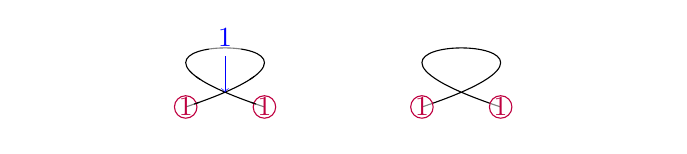
\begin{tikzpicture}
\begin{knot}[
  consider self intersections,
  draft mode=crossings,
]
\strand (0,0) .. controls +(3,1) and +(-3,1) .. (1,0);
\end{knot}
\begin{knot}[
  xshift=3cm,
  consider self intersections=no splits,
  draft mode=crossings,
]
\strand (0,0) .. controls +(3,1) and +(-3,1) .. (1,0);
\end{knot}
\end{tikzpicture}
\end{example}

Finally, given that TikZ has to do some heavy computation to find the intersections, it is worth considering using the \Verb+external+ library of TikZ to avoid having to do this on every run.

\section{Usage}

\subsection{The \texttt{knot} Environment}

\DescribeMacro{knot}
\DescribeMacro{\strand}
This package provides a \Verb+knot+ environment for including in a \Verb+tikzpicture+ to render a knot.
This takes an optional argument which is passed to \Verb+\tikzset+ and can be used to configure the knot.
Within that environment, specific strands are defined using the \Verb+\strand+ command (in place of a \Verb+\path+ or \Verb+\draw+).
Further keys can be specified on the strands.

\DescribeMacro{flip crossing}
\DescribeMacro{\flipcrossings}
Specifying the crossings to be flipped can be done either using the key \Verb+flip crossing+ or the macro \Verb+\flipcrossings+.
The latter can take a comma separated list of crossings to flip.
The former takes a single crossing but can be extended to a comma separated list using the \Verb+.list+ handler as in \Verb+flip crossing/.list={1,2,3}+ (this is what \Verb+\flipcrossings+ does internally).

\DescribeMacro{\redraw}
There is also a macro \Verb+\redraw+ which redraws a strand in the neighbourhood of a point.
This is effectively what happens for the crossings and can be used to fix something that wasn't done correctly by the main algorithm.
It takes two arguments, the strand number and the point at which to render the strand, as in \Verb+\redraw{2}{(1,1)}+.

\subsection{Keys}

The various keys are as follows.
The majority of the keys are in the \Verb+/tikz/knot diagram+ family, but it does its best to pass unknown keys down to \Verb+/tikz/+.
The keys processed by the \Verb+knot+ environment are automatically in this family but the keys processed by the \Verb+\strand+ command are not.
If a standard key (in the option to the \Verb+knot+ environment) doesn't work, try prefixing it with \Verb+/tikz/+ or \Verb+/pgf/+.

\begin{itemize}
\item \DescribeMacro{every knot diagram}
The style \Verb+every knot diagram+ is executed at the start of the \Verb+knot+ environment.

Note that it is inside the \Verb+knot diagram+ family so if setting it outside (say, in the preamble) use \Verb+\tikzset{knot diagram/every knot diagram}+.

\item \DescribeMacro{name}
The crossings of a knot are given coordinates of the form \Verb+<name> <number>+.
The default name is \Verb+knot+.
The \Verb+name+ key renames it.

\item \DescribeMacro{every strand}
The contents of \Verb+every strand+ are applied to every strand.
By default this contains the \Verb+draw+ key so if resetting it you should probably ensure that it still has the \Verb+draw+ key.

Note that it is inside the \Verb+knot diagram+ family so if setting it outside (say, in the preamble) use \Verb+\tikzset{knot diagram/every knot diagram}+.

\item \DescribeMacro{only when rendering}
The key \Verb+only when rendering={<style>}+ is applied to the strand only when it is actually drawn and not when it is used to cut out part of the underlying path.

Note that there are actually two versions of this key: one in the \Verb+knot diagram+ family and one in the \Verb+/tikz+ family.
This is so that it works equally well in the argument to the \Verb+knot+ environment and the \Verb+\strand+ command.

\item \DescribeMacro{ignore endpoint intersections}
When a strand is split into pieces then the intersection library finds ``false positives'' in that neighbouring pieces intersect at their endpoints.
The code ignores such intersections between neighbouring pieces.
The \Verb+ignore endpoint intersections+ (which is true by default) means that all intersections that are near an endpoint are ignored whether or not they are with the next or previous piece of that strand.
The celtic knot example of the previous section sets this to false to ensure that it gets all intersections.

\item \DescribeMacro{consider self intersections}
The key \Verb+consider self intersections=<option>+ handles the splitting facility so that strands can self intersect.
The options are \Verb+true+, \Verb+false+, and \Verb+no splits+.
It is \Verb+false+ at the start, and the default option is \Verb+true+.
The difference between \Verb+true+ and \Verb+no splits+ is as to whether segments are further split to avoid \emph{all} self intersections.

\item \DescribeMacro{clip radius}
The \Verb+clip radius=<length>+ is the radius of the clip region around each crossing.

\item \DescribeMacro{end tolerance}
The \Verb+end tolerance=<length>+ is the distance at which an intersection is considered as being near an endpoint (for simplicity, it uses the \(\ell^1\)--metric).

\item \DescribeMacro{clip width}
The \Verb+clip width=<factor>+ is the multiplier for the thickness of the ``wipeout'' path relative to the line width of the actual path.

\item \DescribeMacro{flip crossing}
The \Verb+flip crossing=<number>+ key flips the \Verb+<number>+ crossing.

\item \DescribeMacro{background colour} \DescribeMacro{background color}
The keys \Verb+background colour=<colour>+ and  \Verb+background color=<color>+ set the background colour for the crossings.

\item \DescribeMacro{every intersection>} \DescribeMacro{intersection <number>}
The style in \Verb+every intersection+ is applied before rendering each crossing, with \Verb+intersection <number>+ applied just before that specific crossing.
These can be used to change how the over-strands are rendered when they are redrawn.
For an example on using \Verb+every intersection+, see Section~\ref{sec:celtic}.


\item \DescribeMacro{draft mode}
The key \Verb+draft mode=<option>+ sets the different styles for aiding with rendering the knot.
The options are \Verb+strands+, \Verb+crossings+, or \Verb+off+.
The \Verb+strands+ option just renders the strands with no crossings.
The \Verb+crossings+ option renders the crossings and labels the strands and crossings.
The \Verb+off+ option renders the crossings without the labels.

\item \DescribeMacro{draft/crossing label}
The style \Verb+draft/crossing label+ is applied to each of the crossing labels.
The labels are actually \Verb+pin+s attached to coordinates at the crossings.
This style is applied to the \Verb+pin+ itself.
The default is:

\begin{lstlisting}
overlay,
fill=white,
fill opacity=.5,
text opacity=1,
text=blue,
pin edge={blue,<-}
\end{lstlisting}

\item \DescribeMacro{draft/strand label}
The style \Verb+draft/strand label+ is applied to each of the strand labels.
The default is:

\begin{lstlisting}
overlay,
circle,
draw=purple,
fill=white,
fill opacity=.5,
text opacity=1,
text=purple,
inner sep=0pt
\end{lstlisting}
\end{itemize}


\subsection{Celtic Knots}
\label{sec:celtic}

By ``Celtic knot'' here, I mean a knot drawn in a way to suggest a carved object.
Usually, this is achieved by using the \Verb+double+ style to outline the path.
This interacts a little oddly with how the knots package redraws the curve near crossings which can result in small artefacts visible when the diagram is viewed (my understanding is that they are not present when the diagram is printed).
There is, however, a way to get these diagrams right, as this section will show.

I will just note here that there is the \href{celtic knots}{https://ctan.org/pkg/celtic} package which works for a particular type of Celtic knots.
If your Celtic knot fits what that package can produce, it is a better choice.
See that package for details.

Back to what this package can provide.
When rendering a crossing, the over-strand is redrawn clipped to a small region around the crossing.
The clipping, however, interacts badly with the \Verb+double+ effect.
The \Verb+double+ effect is achieved by drawing the line twice, once thicker with the outer colour and once thinner with the inner colour.
At the boundary of the clipping region there is ``bleed through'' of the outer colour into the inner colour, at least when the image is displayed on a screen.
If the inner colour is darker, this is not noticeable.
But with a Celtic style knot then the inner colour is usually a lighter colour, such as the page colour, and so the effect is visible.

The solution to this is to exploit the fact that when using the Celtic style then one doesn't actually want gaps in the under-strand to show that it is the under-strand.
The Celtic style makes it very obvious which strand is which without that.
These gaps are achieved by drawing the over-strand in a thicker line with the colour of the background.
This is almost exactly what the \Verb+double+ key does.
So rather than using the \Verb+double+ key directly, we use the mechanism of how the knot crossings are rendered to reproduce the effect.
This avoids the artefacts because when the knot library draws the two paths then it clips them to slightly different sized regions.

\begin{example}
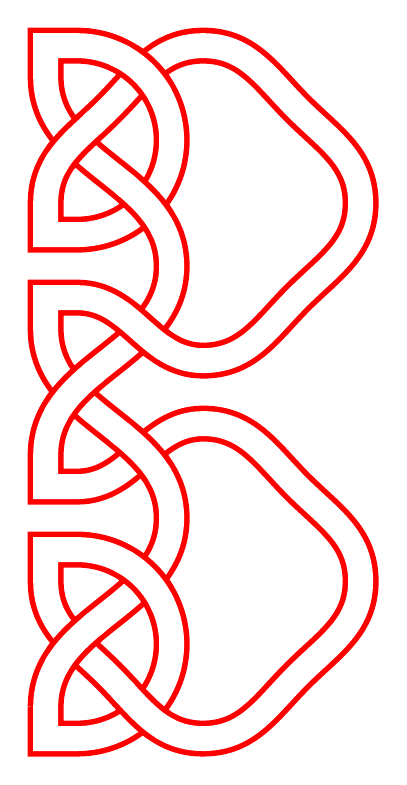
\begin{tikzpicture}[scale=0.8]
\begin{knot}[
  consider self intersections=no splits,
  end tolerance=1pt,
  line join=round,
  clip width=1,
  ignore endpoint intersections=true,
  background color=red,
  every intersection/.style={
    line width=13pt,
    only when rendering/.style={
      draw=white,
      line width=9pt,
      double=none,
    }
  },
  only when rendering/.style={
    red,
    line width=2pt,
    double=white,
    double distance=9pt,
  },
  flip crossing/.list={2,3,6,8}
]

\strand
(0.5,1) to [out=north, in=south]
(2.5,4) to [out=north, in=south]
(0.5,7) -- (0.5,7) -- (0.5,7.5) --
(1,7.5) to [out=east, in=west]
(3,6.5) to [out=east, in=225]
(4.5,7.5) to [out=45, in=south]
(5.5,9) to [out=north, in=-45]
(4.5,10.5) to [out=135,in=east]
(3,11.5) to [out=west,in=45]
(1.5,10.5) to [out=225,in=north]
(0.5,9) -- (0.5,8.5) --
(1,8.5) to [out=east, in=south]
(2.5,10) to [out=north, in=east]
(1,11.5) -- (0.5,11.5) --
(0.5,11) to [out=south, in=north]
(2.5,8) to [out=south, in=north]
(0.5,5) -- (0.5,4.5) --
(1,4.5) to [out=east, in=west]
(3,5.5) to [out=east, in=135]
(4.5,4.5) to [out=-45, in=north]
(5.5,3) to [out=south, in=45]
(4.5,1.5) to [out=225, in=east]
(3,0.5) to [out=west, in=-45]
(1.5,1.5) to [out=135, in=south]
(0.5,3) -- (0.5,3.5) --
(1,3.5) to [out=east, in=north]
(2.5,2) to [out=south, in=east]
(1,0.5) -- (0.5,0.5) -- (0.5,1);
\end{knot}

\end{tikzpicture}

\end{example}






\subsection{Other Styles}

The other things defined by this package are for drawing knot diagrams when the user knows in advance either the locations of the crossings or can arrange that the paths are drawn in the correct order.
In these circumstances the \Verb+knot+ environment is overkill.

\DescribeMacro{knot}
\DescribeMacro{knot gap}
This \Verb+knot=<colour>+ style sets up a doubled path with inner colour the given colour (or the current draw colour if not given) and outer colour the knot background colour.
The width of the inner line is the current line width and the full width is controlled by the \Verb+knot gap=<factor>+ key which is initially set to \(3\) (thus giving a line's width either side).

\begin{example}
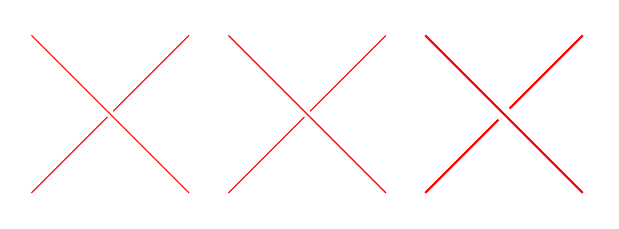
\begin{tikzpicture}[knot gap=7]
\draw[thin,knot=red] (-1,-1) -- (1,1);
\draw[thin,knot=red] (-1,1) -- (1,-1);
\begin{scope}[xshift=2.5cm]
\draw[knot=red] (-1,-1) -- (1,1);
\draw[knot=red] (-1,1) -- (1,-1);
\end{scope}
\begin{scope}[xshift=5cm]
\draw[thick,knot=red] (-1,-1) -- (1,1);
\draw[thick,knot=red] (-1,1) -- (1,-1);
\end{scope}
\end{tikzpicture}
\end{example}

\DescribeMacro{knot crossing}
\DescribeMacro{knot over cross}
\DescribeMacro{knot under cross}
\DescribeMacro{knot horiz}
\DescribeMacro{knot vert}
This package also defines some node shapes to help draw knot and link diagrams.
The idea with these is to place a node of the appropriate type at each crossing and then link them accordingly.
The node shapes are \Verb+knot crossing+, \Verb+knot over cross+, \Verb+knot under cross+, \Verb+knot vert+, \Verb+knot horiz+.
The two styles \Verb+knot over cross+ and \Verb+knot under cross+  are crossings, \Verb+knot vert+ and \Verb+knot horiz+ are for when resolving the crossings in a diagram.
By judicious use of the \Verb+\foreach+ command, a family of resolved link diagrams can be produced.

\begin{example}
\begin{tikzpicture}[every node/.style={draw,red}]
\node[knot over cross] at (1,0) {};
\node[knot under cross] at (2,0) {};
\node[knot vert] at (3,0) {};
\node[knot horiz] at (4,0) {};
\end{tikzpicture}
\end{example}

The node \Verb+knot crossing+ is not meant to be drawn, it is an empty shape.
Its value is in that it defines more anchors than the usual  rectangle shape.
For each of the 8 main compass directions, it defines anchors at 2, 4, 8, 16, and 32 times further out.
This can be useful for designing curves that enter and exit the crossing gracefully at particular directions.
When using this node shape, the crossing itself is easiest to draw by using the \Verb+center+ anchor for the strands that form the over cross.

\begin{example}
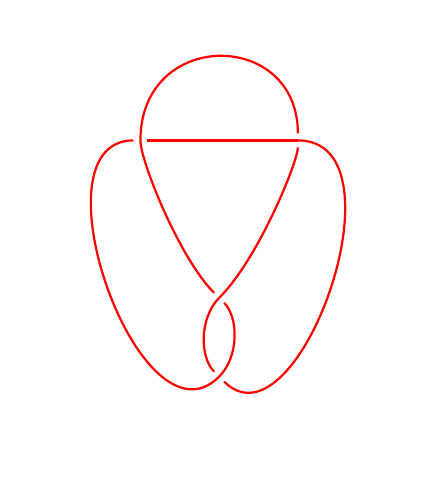
\begin{tikzpicture}[every path/.style={red,thick}, every node/.style={transform shape, knot crossing, inner sep=1.5pt}]
\node[rotate=45] (tl) at (-1,1) {};
\node[rotate=-45] (tr) at (1,1) {};
\node (m) at (0,-1) {};
\node (b) at (0,-2) {};
\draw (b) .. controls (b.4 north west) and (m.4 south west) ..  (m.center);
\draw (b.center) .. controls (b.4 north east) and (m.4 south east) ..  (m);
\draw (m) .. controls (m.8 north west) and (tl.3 south west) ..  (tl.center);
\draw (m.center) .. controls (m.8 north east) and (tr.3 south east) ..  (tr);
\draw (tl.center) .. controls (tl.16 north east) and (tr.16 north  west) .. (tr);
\draw (b) .. controls (b.16 south east) and (tr.16 north east) ..  (tr.center);
\draw (b.center) .. controls (b.16 south west) and (tl.16 north west)  .. (tl);
\draw (tl) -- (tr.center);
\end{tikzpicture}
\end{example}

\section{Other Relevant Packages by the Same Author}

Another tool for drawing knot diagrams is provided by the \Verb+hobby+ package which draws smooth curves through a prescribed set of points.
This can be combined with the facilities of this package but also has some features of its own that make it suitable for drawing knot diagrams.

For braids themselves, there is the \Verb+braids+ package which allows input specification in the form of a word in the braid group.

\end{document}
% Local Variables:
% tex-output-type: "pdf18"
% End:
